
\fullcite{moql07}


\begin{multicols}{2}
\begin{center}
{\bf Article excerpts}
\\ 
{\bf Notes and remarks}
\end{center}
\end{multicols}


\begin{multicols}{2}
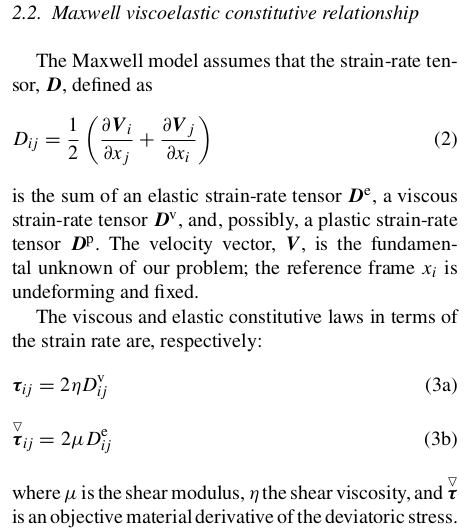
\includegraphics[width=8.25cm]{images/viscoelasticity/moql07a}\\
\[
\dot{\bm\varepsilon}=\frac12
(\vec\nabla \vec\upnu + \vec\nabla \vec\upnu ^T )
\]
\[
{\bm \tau}=2\eta \dot{\bm\varepsilon}_{\rm v}
\]
\[
\check{\bm \tau}=2\mu \dot{\bm\varepsilon}_{\rm e}
\]
where $\check{\bm\tau}$ is an objective material derivative of the deviatoric stress.

\end{multicols}

\begin{multicols}{2}
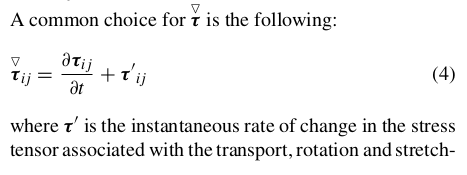
\includegraphics[width=8.25cm]{images/viscoelasticity/moql07b}\\
A common choice for $\check{\bm\tau}$ is the following:
\[
\check{\bm \tau} = \frac{\partial {\bm \tau}}{\partial t}
+ (\vec\upnu\cdot \vec\nabla) {\bm \tau} 
+ {\bm \tau}\cdot \dot{\bm\omega} - \dot{\bm\omega}\cdot {\bm \tau}
+ a ( {\bm \tau} \cdot \dot{\bm\varepsilon} +  \dot{\bm\varepsilon} \cdot {\bm \tau} )
\]
with $-1 \le a \le 1$.
\end{multicols}

\begin{multicols}{2}
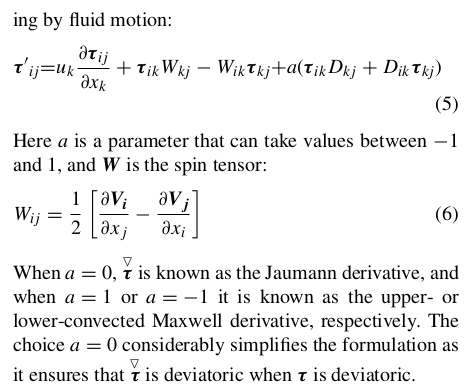
\includegraphics[width=8.25cm]{images/viscoelasticity/moql07c}\\
\[
\dot{\bm\varepsilon} = \dot{\bm\varepsilon}^e+ \dot{\bm\varepsilon}^v
= \frac{\check{\bm \tau}}{2\mu} + \frac{{\bm \tau}}{2\eta}
\]
\end{multicols}

\newpage
\begin{multicols}{2}
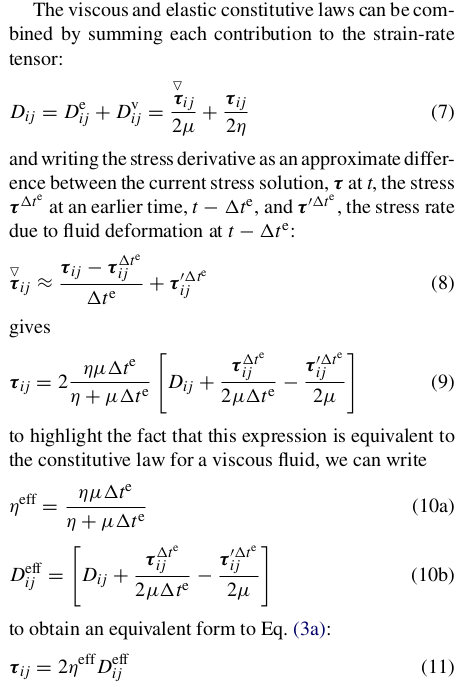
\includegraphics[width=8.25cm]{images/viscoelasticity/moql07d} \\
\[
\dot{\bm\varepsilon} 
= \dot{\bm\varepsilon}_{\rm e} + \dot{\bm\varepsilon}_{\rm v} 
= \frac{\tilde{\bm \tau}  }{2\mu} + \frac{ {\bm \tau}}{2\eta}
\]

\[
\tilde{\bm \tau}^{k+1} \simeq \frac{ {\bm\tau}^{k+1}-{\bm\tau}^k }{\delta t} + \underline{\bm\tau}^k
\]

\[
{\bm\tau} = 2 \frac{\eta \mu \delta t}{\eta + \mu  \delta t}
\left(
\dot{\bm\varepsilon}  + \frac{{\bm\tau}^k}{2\mu \delta t} - \frac{\underline{\bm\tau}^k}{2\mu}
\right)
\]

\[
\eta_{ve} = \frac{\eta \mu \delta t}{\eta + \mu  \delta t}
\]

\end{multicols}
